\documentclass{article}

\usepackage[utf8]{inputenc}
\usepackage{amsmath}
\usepackage{amssymb}
\usepackage{anysize}
\usepackage{color}
\usepackage{xcolor}
\usepackage{graphicx}
\usepackage{float}

\usepackage{listings}
\lstset{
	language=C++,                	% choose the language of the code
	basicstyle=\footnotesize,       % the size of the fonts that are used for the code
	numbers= left,                 	% where to put the line-numbers
	numberstyle=\footnotesize,      % the size of the fonts that are used for the line-numbers
	stepnumber=1,                   % the step between two line-numbers. If it is 1 each line will be numbered
	numbersep=5pt,                  % how far the line-numbers are from the code
	backgroundcolor=\color{white},  % choose the background color. You must add \usepackage{color}
	showspaces=false,               % show spaces adding particular underscores
	showstringspaces=false,         % underline spaces within strings
	showtabs=false,                 % show tabs within strings adding particular underscores
	frame=single,           		% adds a frame around the code
	tabsize=2,          			% sets default tabsize to 2 spaces
	captionpos=t,          			% sets the caption-position to bottom (t=top, b=bottom)
	breaklines=true,        		% sets automatic line breaking
	breakatwhitespace=false,    	% sets if automatic breaks should only happen at whitespace
	escapeinside={\%*}{*)}          % if you want to add a comment within your code
}



\usepackage{caption}
\DeclareCaptionFont{white}{\color{white}}
\DeclareCaptionFormat{listing}{\colorbox{gray}{\parbox[c]{\textwidth}{#1#2#3}}}
\captionsetup[lstlisting]{format=listing,labelfont=white,textfont=white}

\setlength\parindent{0pt}
\setlength{\parskip}{10pt}

\marginsize{3cm}{2cm}{2cm}{2cm}

\title{Software Engineering\\
		Lab 5 Report}
\author{Emre Ozan Alkan\\
		\{emreozanalkan@gmail.com\}\\
		MSCV-5}
\date{15 November 2013}

\begin{document}
\maketitle

\section{Introduction}
Representing cubical model with the Baumgart's winged-edge data structure.

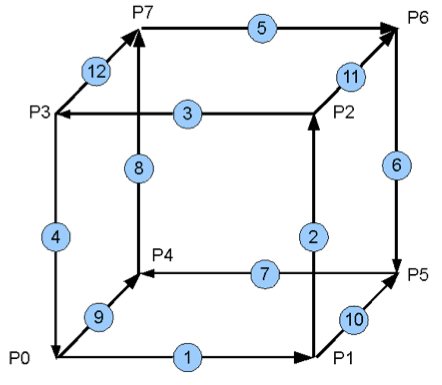
\includegraphics{lab5Cubic.png}

\section{Edge Table}
Edges represented in data structure hold following information;
\begin{enumerate}
\item vertices of this edge, P1 and P2
\item its left and right faces, F1 and F2
\item predecessor(Predccw) and successor(Nextccw) when traversing its left face(ccw)
\item predecessor(Predcw) and successor(Nextcw) when traversing its right face(cw)
\end{enumerate}

Here is the Edge Table following representing closed cubic:


\begin{table}[H]
\centering
    \begin{tabular}{|l|l|l|l|l|l|l|l|l|}
    \hline
    Edge Nb & Start Pt & End Pt & Face ccw F1 & Face cw F2 & Nccw & Pccw & Ncw & Pcw \\ \hline
    1       & P0       & P1     & F1          & F3         & 2    & 4    & 10  & 9   \\ \hline
    2       & P1       & P2     & F1          & F4         & 3    & 1    & 11  & 10  \\ \hline
    3       & P2       & P3     & F1          & F5         & 4    & 2    & 12  & 11  \\ \hline
    4       & P3       & P0     & F1          & F6         & 1    & 3    & 9   & 12  \\ \hline
    5       & P7       & P6     & F2          & F5         & 6    & 8    & 11  & 12  \\ \hline
    6       & P6       & P5     & F2          & F4         & 7    & 5    & 10  & 11  \\ \hline
    7       & P5       & P4     & F2          & F3         & 8    & 6    & 9   & 10  \\ \hline
    8       & P4       & P7     & F2          & F6         & 5    & 7    & 12  & 9   \\ \hline
    9       & P0       & P4     & F3          & F6         & 7    & 1    & 8   & 4   \\ \hline
    10      & P1       & P5     & F4          & F3         & 6    & 2    & 7   & 1   \\ \hline
    11      & P2       & P6     & F5          & F4         & 5    & 3    & 6   & 2   \\ \hline
    12      & P3       & P7     & F6          & F5         & 8    & 4    & 5   & 3   \\ \hline
    \end{tabular}
    \caption {Edge Table}
\end{table}

\section{Face Table}

A faces are represented only with storing start edge, here is the closed cubic representation data for faces:

\begin{table}[H]
\centering
    \begin{tabular}{|c|c|c|c|c|c|}
    \hline
    Face & Point 1 & Point 2 & Point 3 & Point 4 & Start Edge \\ \hline
    F1   & P0      & P1      & P2      & P3      & 1          \\ \hline
    F2   & P7      & P6      & P5      & P4      & 5          \\ \hline
    F3   & P0      & P4      & P5      & P1      & 9          \\ \hline
    F4   & P1      & P5      & P6      & P2      & 10         \\ \hline
    F5   & P2      & P6      & P7      & P3      & 11         \\ \hline
    F6   & P3      & P7      & P4      & P0      & 12         \\ \hline
    \end{tabular}
    \caption {Face Table}
\end{table}


\section{Exercise 1}

In this example, we filled the table of edges(Table 1) in lab.

\section{Exercise 2}

There are 6 class available for representing winged-edge data structure: Point, Edge, Face, ArrayPoint, ArrayEdge, ArrayFace.

\begin{itemize}
\item class Point: Representing a 3D point.
\item class Edge:  Representing edge with 2 points, 2 face ans also 2 previous and 2 next edges in data structure.
\item class Face: Representing a face with start edge.
\item class ArrayPoint: Collection of points.
\item class ArrayEdge: Collection of edges.
\item class ArrayFace: Collection of faces.
\end{itemize}

In header files, there are always \#ifndef, \#define, and \#endif statements for compile time check for multiple file inclusions that protecting including same header files more than once.

In main program, we can add points. edges and faces using menu selection 1, 4 and 10, respectively.

Displaying points, edges and faces can be accomplish by using menu 3, 6, 12, respectively.

Classes are built to handle or keep track of arrays of pointers, by using <type>**.

In order to achieve accomplishment in this lab, it looks like we should implement our function to array class, and call them from the menu.

\section{Exercise 3}

Implemented 2 functions in ArrayEdge, for menu 7 and 8; and implemented 3 function in ArrayFace to provide menu 9 and 13.

\begin{lstlisting}[label=exercice-h, caption=Exercice.h]	

// To class ArrayEdge following public function declarations added
    // "7 : Link segment clockwise - prev and next - (student work here)"
    void linkSegmentsCWCubic(ArrayPoint*);

    // "8 : Link segment counterclockwise - prev and next - (student work here)"
    void linkSegmentsCCWCubic(ArrayPoint*);
    
// To class ArrayFace-to keep coherence- following public functions declarations added
    // "9 : Link segment to faces (student work here)"
    void linkSegmentsToFacesCubic(ArrayEdge*);

    // 13 : Check if face is closed (student work here)"
    bool isCubicFaceClosed() const;
    
// and private function for face traversing
	bool isCubicFaceClosedTraversal(Face*, int) const;

\end{lstlisting}


\null







 

\begin{lstlisting}[label=exercice-cpp, caption=Exercice.cpp]	

// "7 : Link segment clockwise - prev and next - (student work here)"
void ArrayEdge::linkSegmentsCWCubic(ArrayPoint* pointArray)
{
    if(pointArray->n < 8)
    {
        cerr<<"In Point Array, there is not enough element to represent cube."<<endl;
        return;
    }

    Edge* edge01;
    Edge* edge02;
    Edge* edge03;
    Edge* edge04;
    Edge* edge05;
    Edge* edge06;
    Edge* edge07;
    Edge* edge08;
    Edge* edge09;
    Edge* edge10;
    Edge* edge11;
    Edge* edge12;

    if(this->n < 12)
    {
        edge01 = new Edge(pointArray->GetAt(0), pointArray->GetAt(1));
        edge02 = new Edge(pointArray->GetAt(1), pointArray->GetAt(2));
        edge03 = new Edge(pointArray->GetAt(2), pointArray->GetAt(3));
        edge04 = new Edge(pointArray->GetAt(3), pointArray->GetAt(0));
        edge05 = new Edge(pointArray->GetAt(7), pointArray->GetAt(6));
        edge06 = new Edge(pointArray->GetAt(6), pointArray->GetAt(5));
        edge07 = new Edge(pointArray->GetAt(5), pointArray->GetAt(4));
        edge08 = new Edge(pointArray->GetAt(4), pointArray->GetAt(7));
        edge09 = new Edge(pointArray->GetAt(0), pointArray->GetAt(4));
        edge10 = new Edge(pointArray->GetAt(1), pointArray->GetAt(5));
        edge11 = new Edge(pointArray->GetAt(2), pointArray->GetAt(6));
        edge12 = new Edge(pointArray->GetAt(3), pointArray->GetAt(7));

        this->AddEdge(edge01);
        this->AddEdge(edge02);
        this->AddEdge(edge03);
        this->AddEdge(edge04);
        this->AddEdge(edge05);
        this->AddEdge(edge06);
        this->AddEdge(edge07);
        this->AddEdge(edge08);
        this->AddEdge(edge09);
        this->AddEdge(edge10);
        this->AddEdge(edge11);
        this->AddEdge(edge12);
    }
    else
    {
        edge01 = this->GetAt(0);
        edge02 = this->GetAt(1);
        edge03 = this->GetAt(2);
        edge04 = this->GetAt(3);
        edge05 = this->GetAt(4);
        edge06 = this->GetAt(5);
        edge07 = this->GetAt(6);
        edge08 = this->GetAt(7);
        edge09 = this->GetAt(8);
        edge10 = this->GetAt(9);
        edge11 = this->GetAt(10);
        edge12 = this->GetAt(11);
    }

    edge01->Nextcw  = edge10;
    edge01->Prevcw  = edge09;

    edge02->Nextcw  = edge11;
    edge02->Prevcw  = edge10;

    edge03->Nextcw  = edge12;
    edge03->Prevcw  = edge11;

    edge04->Nextcw  = edge09;
    edge04->Prevcw  = edge12;

    edge05->Nextcw  = edge11;
    edge05->Prevcw  = edge12;

    edge06->Nextcw  = edge10;
    edge06->Prevcw  = edge11;

    edge07->Nextcw  = edge09;
    edge07->Prevcw  = edge10;

    edge08->Nextcw  = edge12;
    edge08->Prevcw  = edge09;

    edge09->Nextcw  = edge08;
    edge09->Prevcw  = edge04;

    edge10->Nextcw  = edge07;
    edge10->Prevcw  = edge01;

    edge11->Nextcw  = edge06;
    edge11->Prevcw  = edge02;

    edge12->Nextcw  = edge05;
    edge12->Prevcw  = edge03;

    return;
}

// "8 : Link segment counterclockwise - prev and next - (student work here)"
void ArrayEdge::linkSegmentsCCWCubic(ArrayPoint* pointArray)
{
    if(pointArray->n < 8)
    {
        cerr<<"In Point Array, there is not enough element to represent cube."<<endl;
        return;
    }

    Edge* edge01;
    Edge* edge02;
    Edge* edge03;
    Edge* edge04;
    Edge* edge05;
    Edge* edge06;
    Edge* edge07;
    Edge* edge08;
    Edge* edge09;
    Edge* edge10;
    Edge* edge11;
    Edge* edge12;

    if(this->n < 12)
    {
        edge01 = new Edge(pointArray->GetAt(0), pointArray->GetAt(1));
        edge02 = new Edge(pointArray->GetAt(1), pointArray->GetAt(2));
        edge03 = new Edge(pointArray->GetAt(2), pointArray->GetAt(3));
        edge04 = new Edge(pointArray->GetAt(3), pointArray->GetAt(0));
        edge05 = new Edge(pointArray->GetAt(7), pointArray->GetAt(6));
        edge06 = new Edge(pointArray->GetAt(6), pointArray->GetAt(5));
        edge07 = new Edge(pointArray->GetAt(5), pointArray->GetAt(4));
        edge08 = new Edge(pointArray->GetAt(4), pointArray->GetAt(7));
        edge09 = new Edge(pointArray->GetAt(0), pointArray->GetAt(4));
        edge10 = new Edge(pointArray->GetAt(1), pointArray->GetAt(5));
        edge11 = new Edge(pointArray->GetAt(2), pointArray->GetAt(6));
        edge12 = new Edge(pointArray->GetAt(3), pointArray->GetAt(7));

        this->AddEdge(edge01);
        this->AddEdge(edge02);
        this->AddEdge(edge03);
        this->AddEdge(edge04);
        this->AddEdge(edge05);
        this->AddEdge(edge06);
        this->AddEdge(edge07);
        this->AddEdge(edge08);
        this->AddEdge(edge09);
        this->AddEdge(edge10);
        this->AddEdge(edge11);
        this->AddEdge(edge12);
    }
    else
    {
        edge01 = this->GetAt(0);
        edge02 = this->GetAt(1);
        edge03 = this->GetAt(2);
        edge04 = this->GetAt(3);
        edge05 = this->GetAt(4);
        edge06 = this->GetAt(5);
        edge07 = this->GetAt(6);
        edge08 = this->GetAt(7);
        edge09 = this->GetAt(8);
        edge10 = this->GetAt(9);
        edge11 = this->GetAt(10);
        edge12 = this->GetAt(11);
    }

    edge01->Nextccw  = edge02;
    edge01->Prevccw  = edge04;

    edge02->Nextccw  = edge03;
    edge02->Prevccw  = edge01;

    edge03->Nextccw  = edge04;
    edge03->Prevccw  = edge02;

    edge04->Nextccw  = edge01;
    edge04->Prevccw  = edge03;

    edge05->Nextccw  = edge06;
    edge05->Prevccw  = edge08;

    edge06->Nextccw  = edge07;
    edge06->Prevccw  = edge05;

    edge07->Nextccw  = edge08;
    edge07->Prevccw  = edge06;

    edge08->Nextccw  = edge05;
    edge08->Prevccw  = edge07;

    edge09->Nextccw  = edge07;
    edge09->Prevccw  = edge01;

    edge10->Nextccw  = edge06;
    edge10->Prevccw  = edge02;

    edge11->Nextccw  = edge05;
    edge11->Prevccw  = edge03;

    edge12->Nextccw  = edge08;
    edge12->Prevccw  = edge04;

    return;
}

// "9 : Link segment to faces (student work here)"
void ArrayFace::linkSegmentsToFacesCubic(ArrayEdge* edgeArray)
{
    if(edgeArray->n < 12)
    {
        cerr<<"In Edge Array, there is not enough edge to represent cube."<<endl;
        return;
    }

    Face *F1;
    Face *F2;
    Face *F3;
    Face *F4;
    Face *F5;
    Face *F6;

    if(this->n < 6)
    {
        F1 = new Face;
        F2 = new Face;
        F3 = new Face;
        F4 = new Face;
        F5 = new Face;
        F6 = new Face;

        this->AddFace(F1);
        this->AddFace(F2);
        this->AddFace(F3);
        this->AddFace(F4);
        this->AddFace(F5);
        this->AddFace(F6);
    }
    else
    {
        F1 = this->GetAt(0);
        F2 = this->GetAt(1);
        F3 = this->GetAt(2);
        F4 = this->GetAt(3);
        F5 = this->GetAt(4);
        F6 = this->GetAt(5);
    }

    Edge* edge01 = edgeArray->GetAt(0);
    Edge* edge02 = edgeArray->GetAt(1);
    Edge* edge03 = edgeArray->GetAt(2);
    Edge* edge04 = edgeArray->GetAt(3);
    Edge* edge05 = edgeArray->GetAt(4);
    Edge* edge06 = edgeArray->GetAt(5);
    Edge* edge07 = edgeArray->GetAt(6);
    Edge* edge08 = edgeArray->GetAt(7);
    Edge* edge09 = edgeArray->GetAt(8);
    Edge* edge10 = edgeArray->GetAt(9);
    Edge* edge11 = edgeArray->GetAt(10);
    Edge* edge12 = edgeArray->GetAt(11);

    edge01->Fccw = F1;
    edge01->Fcw =  F3;

    edge02->Fccw = F1;
    edge02->Fcw =  F4;

    edge03->Fccw = F1;
    edge03->Fcw =  F5;

    edge04->Fccw = F1;
    edge04->Fcw =  F6;

    edge05->Fccw = F2;
    edge05->Fcw =  F5;

    edge06->Fccw = F2;
    edge06->Fcw =  F4;

    edge07->Fccw = F2;
    edge07->Fcw =  F3;

    edge08->Fccw = F2;
    edge08->Fcw =  F6;

    edge09->Fccw = F3;
    edge09->Fcw =  F6;

    edge10->Fccw = F4;
    edge10->Fcw =  F3;

    edge11->Fccw = F5;
    edge11->Fcw =  F4;

    edge12->Fccw = F6;
    edge12->Fcw =  F5;

    F1->Start = edge01;
    F2->Start = edge05;
    F3->Start = edge09;
    F4->Start = edge10;
    F5->Start = edge11;
    F6->Start = edge12;

    return;
}

\end{lstlisting}

\section{Exercise 4}
In order to check our cubical is represented closed in our data structure, here are the functions to check it.

\begin{lstlisting}[label=exercices-h-traversal,caption=Exercice.h]	
    // 13 : Check if face is closed (student work here)"
    bool isCubicFaceClosed() const;
    private:
    bool isCubicFaceClosedTraversal(Face*, int) const;
\end{lstlisting}

\begin{lstlisting}[label=exercices-cpp-traversal,caption=Exercice.cpp]	
// 13 : Check if face is closed (student work here)"
bool ArrayFace::isCubicFaceClosed() const
{
    bool isCubicFaceClosed = true;

    for(int i = 0; i < this->n; i++)
    {
        Face* face = this->GetAt(i);

        bool traversal = this->isCubicFaceClosedTraversal(face, 4);

        if(!traversal)
        {
            isCubicFaceClosed = false;
            break;
        }
    }

    return isCubicFaceClosed;
}

bool ArrayFace::isCubicFaceClosedTraversal(Face* face, int numberOfEdges) const
{
    Edge* temp = face->Start;

    for(int i = 0; i < numberOfEdges; i++)
    {
        if(temp->Fccw == face)
            temp = temp->Nextccw;
        else
            temp = temp->Prevcw;
    }

    if(temp == face->Start)
        return true;
    return false;
}
\end{lstlisting}

Here are the some function call from main.cpp

\begin{lstlisting}[label=main-cpp,caption=main.cpp]	

//-------------------------
//student work here
//-------------------------

            case 7 : {
                //add your code here

            // "7 : Link segment clockwise - prev and next - (student work here)"
            ArrayE.linkSegmentsCWCubic(&ArrayP);


                }break;

//-------------------------
//student work here
//-------------------------

            case 8 : {
                //add your code here

            // "8 : Link segment counterclockwise - prev and next - (student work here)"
            ArrayE.linkSegmentsCCWCubic(&ArrayP);


                }break;

//-------------------------
//student work here
//-------------------------

            case 9 : {
                //add your code here

            // "9 : Link segment to faces (student work here)"
            ArrayF.linkSegmentsToFacesCubic(&ArrayE);

                }break;
                
            case 13 : {
                //student work here

            // "13 : Check if face is closed (student work here)"
            bool isClosed = ArrayF.isCubicFaceClosed();
            if(isClosed)
                cout<<"Cubic Faces looks closed ^_^ !"<<endl;
            else
                cout<<"Cubic Faces looks like NOT closed :'( !"<<endl;

                }break;


\end{lstlisting}



\section{Results/Lessons Learned}

This lab gave us the message not to use winged-edge again, otherwise it's data structure is a pain.




\end{document}







































